\documentclass[12pt,a4paper]{article}
\usepackage[utf8]{inputenc}
\usepackage[russian]{babel}
\usepackage[OT1]{fontenc}
\usepackage{amsmath}
\usepackage{amsfonts}
\usepackage{amssymb}
\usepackage{graphicx}
\graphicspath{{Images/}}
\usepackage[left=2cm,right=2cm,top=2cm,bottom=2cm]{geometry}
\usepackage{calc}
\usepackage{wrapfig}
\usepackage{setspace}
\usepackage{indentfirst}
\usepackage{amssymb}
\usepackage{subfigure}
\usepackage{multirow}

\title{
Отчет о выполнении лабораторной работы 3.4.2

Закон Кюри–Вейсса
}

\author{Комкин Михаил, группа Б01-303}
\newpage
\begin{document}

\maketitle
\textbf{Цель работы:} изучение температурной зависимости магнитной восприимчивости ферромагнетика выше точки Кюри.
\\
\\
\textbf{В работе используются:} катушка самоиндукции с образцом из гадолиния, термостат, частотомер, цифровой вольтметр, $LC$-автогенератор, термопара медь–константан.
\\
\\
Вещества с отличными от нуля атомными магнитными моментами
обладают парамагнитными свойствами. Внешнее магнитное поле ориентирует магнитные моменты, которые в отсутствие поля располагались
в пространстве хаотичным образом. При повышении температуры $T$ возрастает дезориентирующее действие теплового движения частиц, и магнитная восприимчивость парамагнетиков убывает по закону Кюри
— обратно пропорционально температуре. 

\[
\chi \propto \frac{1}{T - \Theta_p}
\]

Непосредственно вблизи $\Theta_K$ закон Кюри–Вейсса (2) нарушается. На
практике наблюдается зависимость, изображённая на рис. 1.

\begin{figure}[h!]
	\begin{center}
		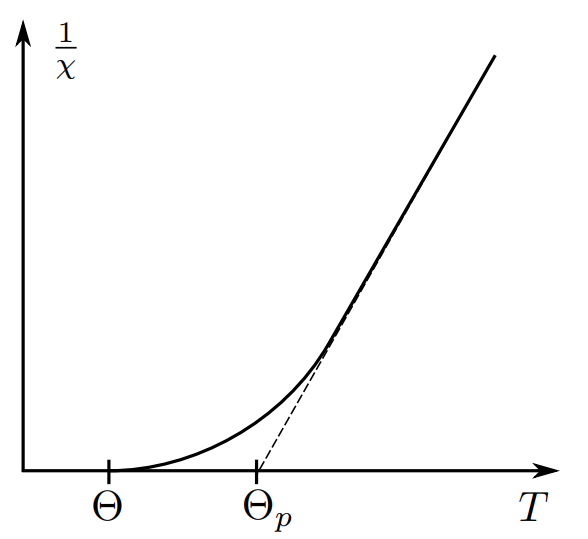
\includegraphics[width = 0.4\textwidth]{image.png}
		\label{fig:facility}
        \caption{Зависимость обратной
        величины магнитной восприимчивости от температуры.}
	\end{center}
\end{figure}

\section{Экспериментальная установка}

В работе изучается температурная зависимость $\chi(T)$ гадолиния при
температурах выше точки Кюри. Выбор материала определяется тем,
что его точка Кюри лежит в диапазоне комнатных температур.
\begin{figure}[h!]
	\begin{center}
		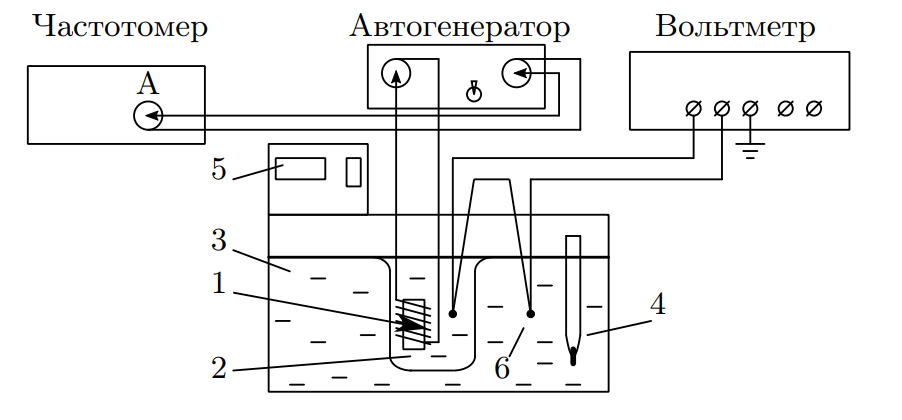
\includegraphics[width = 0.7\textwidth]{ust.png}
		\label{fig:facility}
        \caption{ Схема экспериментальной установки}
	\end{center}
\end{figure}

Схема установки для проверки закона Кюри-Вейса показана на рис. 2. Исследуемый ферромагнитный образец (гадолиний) расположен внутри пустотелой катушки самоиндукции, которая служит индуктивностью колебательного контура, входящего в состав LC-автогенератора (генератора колебаний с самовозбуждением).

Гадолиний является хорошим проводником электрического тока, а рабочая частота генератора достаточно велика (\(\sim 50\ \text{кГц}\)), поэтому для уменьшения вихревых токов образец изготовлен из мелких кусочков размером \(0.5\ \text{мм}\). Катушка 1 с образцом помещена в термостат 3, залитый трансформаторным маслом. Масло предохраняет образец от окисления при высоких температурах. Регулировка температуры осуществляется с помощью нагревателя 4 и термопары. Температура образца регулируется с помощью термостата 5.

Коэффициент самоиндукции катушки \(L\) пропорционален магнитной проницаемости и заполняющей его среды (почему?): \(L \propto \mu\). Тогда разность самоиндукции катушки с образцом \(L\) и без него \(L_0\) будет пропорциональна восприимчивости образца \(\chi\):
\[
L = L_0 \cdot \mu = L_0 \cdot (1 + \chi).
\]

При изменении индуктивности образца меняется период колебаний автогенератора:
\[
\tau = 2 \pi \sqrt{LC},
\]
где \(C\) — ёмкость контура автогенератора. Период колебаний в отсутствие образца определяется самоиндукцией пустой катушки:
\[
\tau_0 = 2 \pi \sqrt{L_0 C}.
\]
Отсюда находим
\[
L = L_0 \cdot \frac{\tau^2}{\tau_0^2},
\]
и, следовательно,
\[
\chi \approx \frac{\tau^2}{\tau_0^2} - 1. \tag{3}
\]

Из формул (2) и (3) следует, что закон Кюри-Вейса справедлив, если выполнено соотношение
\[
\frac{1}{\tau^2 - \tau_0^2} \propto T - \Theta_p. \tag{4}
\]

Измерения проводятся в интервале температур от \(14^\circ C\) до \(40^\circ C\). С целью экономии времени следует начинать измерения с низких температур.



Температура исследуемого образца всегда несколько отличается от
температуры воды в термостате. После того как вода достигла заданной температуры, идёт медленный процесс выравнивания температур
образца и воды. Разность их температур контролируется с помощью
медно-константановой термопары 6, один из спаев которой находится в
тепловом контакте с образцом, а другой погружён в воду. Чувствительность термопары указана на установке. Рекомендуется измерять период
колебаний автогенератора в тот момент, когда указанная разность температур становится меньше $ 0.5^{\circ}  C$ (более точному измерению температур
мешают паразитные ЭДС, возникающие в цепи термопары).




\section{Экспериментальные данные}

Погрешности:
\[
	\Delta T = 0.01
\]
\[
	\Delta \tau = 0.001
\]
\begin{table}[!ht]
    \centering
    \begin{tabular}{|l|l|l|l|}
    \hline
        $T ^\circ C$ & $\tau$,  мкс & $\varepsilon$, мкВ & $\frac{1}{\tau^2 - \tau_0^2}$ \\ \hline
        14.01 & 10.0803 & 20 & 0.546956189 \\ \hline
        16.02 & 9.95619 & 10 & 0.586789032 \\ \hline
        18.02 & 9.7559 & 10 & 0.664937828 \\ \hline
        20.02 & 9.5073 & 20 & 0.796622321 \\ \hline
        22 & 9.06843 & 10 & 1.224844751 \\ \hline
        24 & 8.779850 & 20 & 1.894477598 \\ \hline
        26 & 8.6285 & 20 & 2.656042497 \\ \hline
        28 & 8.544 & 20 & 3.424657534 \\ \hline
        30 & 8.488 & 10 & 4.237288136 \\ \hline
        32 & 8.4568 & 20 & 4.8828125 \\ \hline
        34 & 8.4291 & 10 & 5.646527386 \\ \hline
        36 & 8.4096 & 10 & 6.345177665 \\ \hline
        38 & 8.3943913 & 10 & 7.022900978 \\ \hline
        40 & 8.38194 & 10 & 7.695859628 \\ \hline
    \end{tabular}
\end{table}

\begin{figure}[h!]
	\begin{center}
		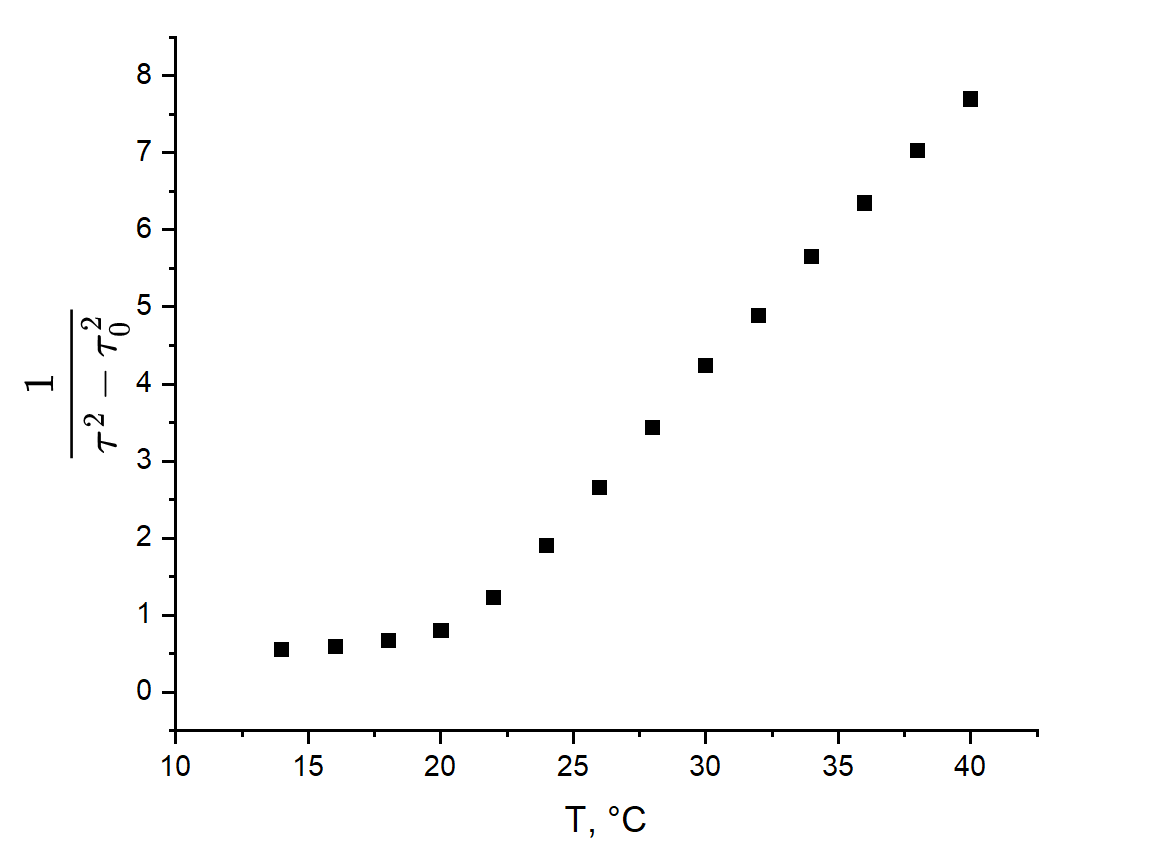
\includegraphics[width = 0.7\textwidth]{full.png}
		\label{fig:facility}
        \caption{Закон Кюри-Вейса}
	\end{center}
\end{figure}

\begin{figure}[h!]
	\begin{center}
		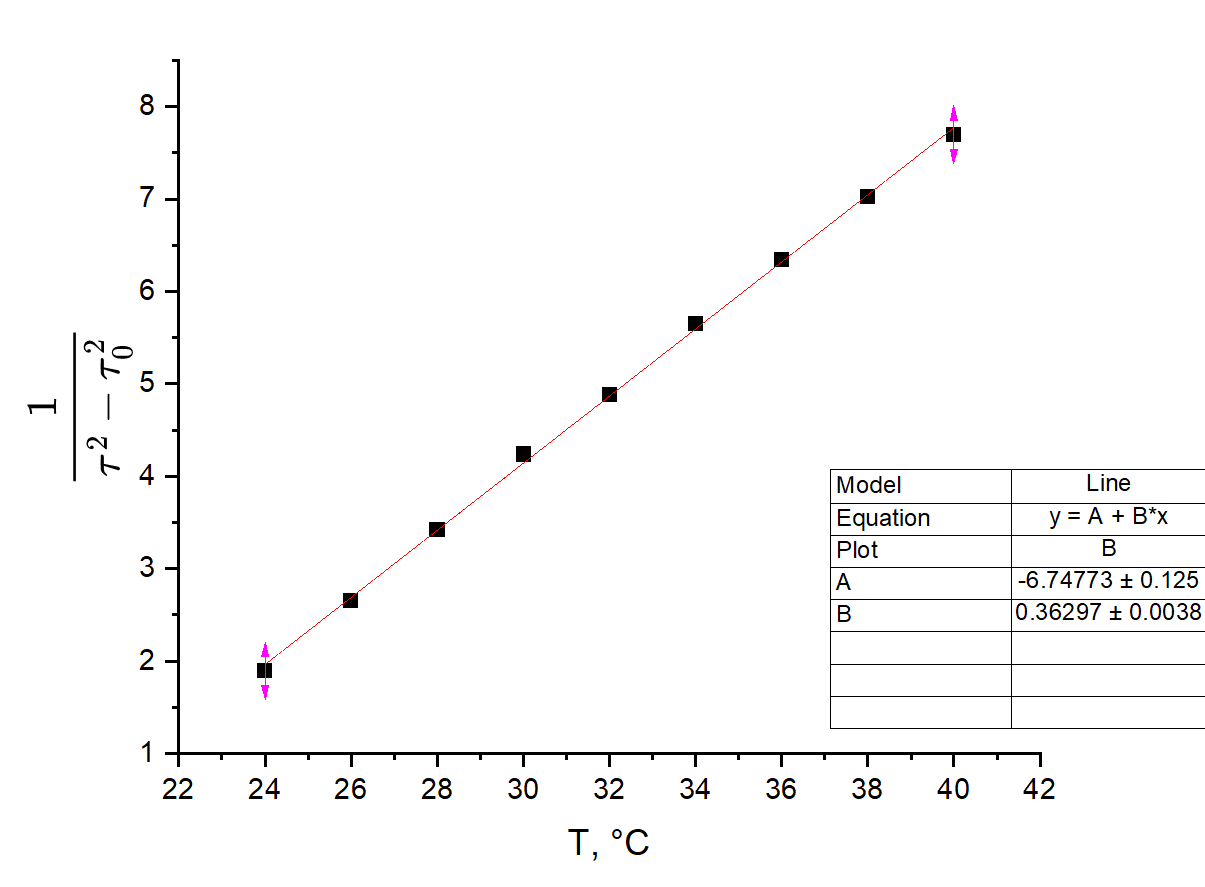
\includegraphics[width = 0.7\textwidth]{line.png}
		\label{fig:facility}
        \caption{Точка Кюри}
	\end{center}
\end{figure}

\[
	\Theta_p = (18.6 \pm 0.2)^\circ C
\]

\[
	\Theta_K \approx (22 \pm 2) ^\circ C
\]
\section{Вывод}

В ходе работы был проверен закон Кюри–Вейсса вблизи точки Кюри и получены значения совпадающие с теоретическими.
Теоретическое значение для температуры Кюри $\Theta_K = 20.2 ^\circ C$. Совпадает с полученным в пределах доверительного интервала.
\end{document}